\section{Noisy Complaint Sets}
\label{sec:noise}

\subsubsection{False Negatives}
False negatives are cases when we don't have the full complaint sets, but
what's provided in the complaint sets are guaranteed as correct. The 
two-iteration approach in Section~\ref{sec:opt:tbsize} can handle 
such cases. Refer to Section~\ref{sec:opt:tbsize} for detail.
\subsubsection{False Positives}
False positives are cases when we have incorrect information in the complaint sets 
: they can be a falsely reported tuple which are actually 
correct, or incorrect suggestions for the erroneous tuples. 
Including such false positives in the MILP problem may result in a problem
that is infeasible to solve. Thus, we want to detect and prune these false positives 
beforehand. However, false positives are hard to 
detect when there is a lack of information. 
For example, if we only have few tuples in the complaint
set, we cannot make any claim about which of them is a false positive 
complaint. Thus, in this paper, we only considering false positive
case when the ratio of the number of false positives to the number
of correctly reported complaints is small.
A obvious trend for false positives is that they normally are very 
different or conflict
with other complaints (Example~\ref{ex:false_positive_1}).
\begin{example} \label{ex:false_positive_1}
In Example~r\ref{ex:taxes2}, say there is 
a false positive complaint on tuple $t_5$ which suggests the correct value
for $t_5$ at database state $D_3$ should be 
\{\textbf{ID}:$t_5$, \textbf{rate}: \color{red}{30}
\color{black}{, \textbf{income}: \$5000, \textbf{owned}
: }\color{red}{\$1500}\color{black}{\}}. To resolve this complaint, we have
to guarantee the lower bound of the income range in $q_1$ as 5000. 
However, the other complaints, $t_1, t_2, t_3$, suggest to
move this lower bound to at least 9500.0001. In this case, the complaint
$t_5$ conflicts with the all the other complaints and we may thus
claim that $t_5$ is likely to be a false positive complaint. 
\end{example}
In this section, we introduce a \textbf{Pre-Processing} process that detects 
false positives effectively. This pre-processing process first searches the 
best log repair for each complaint separately, it then constructs 
a bipartite graph between complaints and their impacted tuples and
searches for the densest sub-graph of the bipartite graph, and finally 
prunes complaints that are not in the densest sub-graph.
\begin{itemize}
\item Using algorithm described in Section~\ref{sec:opt} to solve each 
complaint individually. Denote the log repair for complaint $c_i$ 
as $\mathcal{Q}^*(c_i)$, and the impacted tuples of this log repair as
$T_{c_i}$.
\item Construct a bipartite graph $G = (\mathcal{C}, T, E)$, where 
$T = \cup_{i} T_{c_i}$. Note that tuple with same primary key but modified 
differently are treated as two separate vertices in the bipartite graph. 
\item Search for densest sub-graph $G' = (\mathcal{C}', T', E')$ in $G$ 
[] \xlw{cite some papers} and prune complaints in $\mathcal{C} - \mathcal{C}'$. 
Density[] of a graph $G' = (\mathcal{C}', T', E')$
 is defined by $density(G') = \frac{|E'|}{|\mathcal{C}'|+|T'|}$. 
\end{itemize}
For achieve better performance, we can sample tuples
from the database uniformly when constructing the bipartite graph $G$. 
We demonstrate how to use this \textbf{Pre-Processing} 
approach to prune false positive complaint(s) in Example~\ref{ex:false_positive_2}. 
\begin{example}
\label{ex:false_positive_2}
Let's construct the bipartite graph between complaints $t_1, t_2, t_3, t_5$ 
and tuples in the table for Example~\ref{ex:false_positive_1}. 
$t_1$ suggests to move the range of income in $q_1$ 
as $(9000, 10000]$. Similarly, $t_2, t_3, t_5$ suggest $[8570, 90000]$, 
$[8570, 86000]$, and $[500, 10000]$ respectively. Let's assume tuples are
uniformly distributed in these ranges. The bipartite graph is shown in 
Figure~\ref{f:fp}. The density for $t_2, t_3$ is 1.9202 ($\frac{313}{163}$);
density for $t_2, t_3, t_1$ is 1.9207 ($\frac{315}{164}$); density for 
$t_1, t_2, t_3, t_5$ is 1.8232 ($\frac{330}{181}$). Thus, $t_5$ is pruned. 
\begin{figure}[ht]
\centering
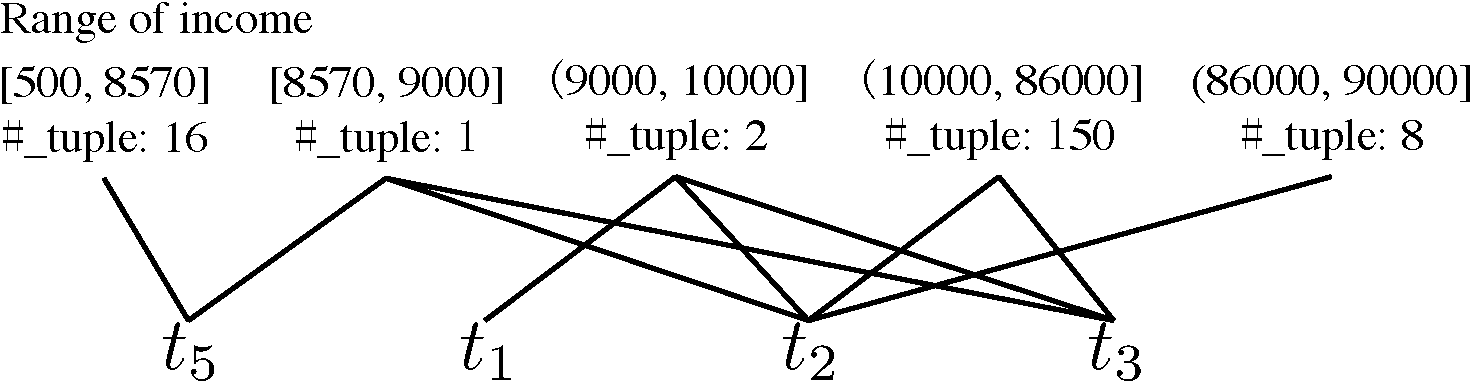
\includegraphics[width = 0.85\columnwidth]{figures/falsepositive_example}
\caption{Bipartite graph of complaints and tuples for Example~\ref{ex:taxes2}. }
\label{f:pf} 
\end{figure}
\end{example}
